\documentclass[11pt,a4paper]{article}
\usepackage[margin=0.85in]{geometry}
\usepackage[T1]{fontenc}
\usepackage{lmodern}
\usepackage{microtype}
\usepackage{enumitem}
\usepackage{booktabs}
\usepackage{longtable}
\usepackage{array}
\usepackage{float}
\usepackage{capt-of}
\usepackage{amsmath}
\usepackage{placeins}
\usepackage{graphicx}
\usepackage{xcolor}
\usepackage{titlesec}
\usepackage{tikz}
\usetikzlibrary{arrows.meta,positioning,shapes.geometric,calc,fit}
\usepackage[hidelinks]{hyperref}
\usepackage{fancyhdr}
\usepackage{lastpage}

% ---------- General layout ----------
\setlength{\parindent}{0pt}
\numberwithin{figure}{section}   % figure numbers follow the format: 1.1, 2.1, 2.2, ...
\setlength{\parskip}{5pt}
\setlength{\headheight}{14pt}
\setlist{nosep,leftmargin=*}
\renewcommand{\arraystretch}{1.15}
\titleformat{\section}{\sffamily\Large\bfseries}{\thesection}{0.8em}{}
\titleformat{\subsection}{\sffamily\large\bfseries}{\thesubsection}{0.8em}{}
\titlespacing*{\section}{0pt}{16pt}{8pt}
\titlespacing*{\subsection}{0pt}{12pt}{6pt}
\pagestyle{fancy}
\fancyhf{}
\lhead{\small SHARP -- Software Requirements Specification}
\rhead{\small UCS503P -- 2026--27 ODD}
\cfoot{\small\thepage\ of \pageref{LastPage}}
\renewcommand{\headrulewidth}{0.4pt}
\hypersetup{pdftitle={SHARP Software Requirements Specification},pdfauthor={SHARP Project Team}}

% ---------- Diagram styles ----------
\tikzset{
  flow/.style={-{Latex},thick},
  dashedflow/.style={-{Latex},thick,dashed},
  flowbox/.style={draw,rounded corners,align=center,text width=40mm,minimum height=8mm,font=\small},
  decision/.style={draw,diamond,aspect=2.4,align=center,inner sep=1pt,font=\small},
  ent/.style={draw,ellipse,align=center,minimum width=28mm,minimum height=11mm,inner sep=2pt,font=\footnotesize\bfseries},
  lbl/.style={midway,fill=white,inner sep=1.5pt,font=\scriptsize,align=center},
  utype/.style={draw,rounded corners,align=center,minimum width=24mm,minimum height=8mm,font=\small\bfseries}
}

% ---------- Data-flow-diagram styles ----------
\tikzset{
  ext/.style={draw,fill=white,align=center,minimum width=26mm,minimum height=10mm,font=\scriptsize\bfseries},
  proc/.style={draw,rounded corners=5pt,fill=gray!10,align=center,text width=32mm,minimum height=18mm,font=\scriptsize\bfseries},
  dl/.style={fill=white,inner sep=1pt,font=\scriptsize,align=center,text width=40mm},
  store/.style={draw=none,text width=44mm,align=left,inner sep=3pt,minimum height=8mm,font=\scriptsize}
}
% Open-ended data store: \dstore{name}{x}{y}{text}
\newcommand{\dstore}[4]{%
  \node[store] (#1) at (#2,#3) {#4};
  \draw (#1.north west) -- (#1.north east);
  \draw (#1.south west) -- (#1.south east);
  \draw (#1.north west) -- (#1.south west);}
% Two-way flow (double-headed arrow): \bflow{from}{to}{label}
\newcommand{\bflow}[3]{\draw[{Latex}-{Latex},thick] (#1) -- node[dl]{#3} (#2);}
\newcommand{\oflow}[3]{\draw[flow] (#1) -- node[dl]{#3} (#2);}

% ---------- Activity-card styles (as in the format's activity figures) ----------
\tikzset{
  chead/.style={draw,fill=black,text=white,text width=40mm,align=center,font=\scriptsize\bfseries,minimum height=6mm,outer sep=0pt},
  citem/.style={draw,text width=40mm,align=center,font=\scriptsize,minimum height=6mm,outer sep=0pt},
  pstep/.style={draw,rounded corners=3pt,fill=white,align=center,text width=17mm,minimum height=11mm,font=\scriptsize,inner sep=2pt}
}
% Role card: \card{id}{x}{y}{title}{{item1},{item2},...}  (alternating shading)
\newcommand{\card}[5]{%
  \node[chead,anchor=north] (#1h) at (#2,#3) {#4};
  \foreach \itm [count=\i] in {#5} {%
    \pgfmathtruncatemacro{\pv}{\i-1}%
    \ifnum\i=1
      \node[citem,below=0pt of #1h,fill=gray!28] (#1\i) {\itm};%
    \else
      \ifodd\i
        \node[citem,below=0pt of #1\pv,fill=gray!28] (#1\i) {\itm};%
      \else
        \node[citem,below=0pt of #1\pv,fill=gray!12] (#1\i) {\itm};%
      \fi
    \fi}}
% Process box with arrow: \procbox{id}{x}{y}{title}{step1}{step2}{step3}  (box is 78mm x 34mm, top-left at x,y)
\newcommand{\procbox}[7]{%
  \draw (#2,#3) rectangle ++(7.8,-3.4);
  \fill[gray!30] ($(#2,#3)+(0.3,-0.55)$) -- ++(6.5,0) -- ++(0,0.3) -- ++(0.75,-1.05) -- ++(-0.75,-1.05) -- ++(0,0.3) -- ++(-6.5,0) -- cycle;
  \node[pstep] at ($(#2,#3)+(1.4,-1.3)$) {#5};
  \node[pstep] at ($(#2,#3)+(3.6,-1.3)$) {#6};
  \node[pstep] at ($(#2,#3)+(5.8,-1.3)$) {#7};
  \node[font=\bfseries\small] at ($(#2,#3)+(3.9,-2.85)$) {#4};
  \coordinate (#1) at ($(#2,#3)+(3.9,-1.7)$);
  \coordinate (#1e) at ($(#2,#3)+(7.8,-1.7)$);
  \coordinate (#1n) at ($(#2,#3)+(3.9,0)$);
  \coordinate (#1s) at ($(#2,#3)+(3.9,-3.4)$);}
% Frame with a bold title underneath: \roleframe{nodes to enclose}{title}
\newcommand{\roleframe}[2]{%
  \node[draw,fit=#1,inner sep=8pt] (frm) {};
  \node[below=3pt of frm,font=\bfseries\small\sffamily] {#2};}

\begin{document}

% ---------- Title page ----------
\begin{titlepage}
\thispagestyle{empty}
\vspace*{0.25in}
\noindent\rule{\textwidth}{1.4pt}
\vspace{0.55in}
\begin{center}
{\Large\bfseries SOFTWARE REQUIREMENTS\\[0.15em] SPECIFICATION}\par
\vspace{0.5in}
{\large for}\par
\vspace{0.4in}
{\LARGE\bfseries SHARP}\par
\vspace{0.15in}
{\large Smart Hostel Administration and Resource Platform}\par
\vspace{0.35in}
{\normalsize\textbf{Submitted by:}}\par
\vspace{0.12in}
\begin{tabular}{ll}
1. Vaibhav Kansal & (1024160097)\\
2. Ayush Kamboj & (1024160118)\\
3. Ali Ekram & (1024160138)\\
4. Riya Gupta & (1024160122)
\end{tabular}\par
\vspace{0.35in}
{\normalsize\textbf{Submitted to:}}\par
\vspace{0.08in}
Ms.~Anushka\par
Course Instructor\par
UCS503P -- Software Engineering Project\par
\vspace{0.25in}
Thapar Institute of Engineering and Technology\par
Session 2026--27 ODD\par
\vspace{0.25in}
October 2026
\end{center}
\vfill
\begin{center}{\small Document status: this SRS describes the planned system and its delivery phases.}\end{center}
\end{titlepage}

\pagenumbering{arabic}
\tableofcontents
\newpage

% =====================================================================
\section{Introduction}
\subsection{Purpose}
This Software Requirements Specification (SRS) defines the main functions, users, operating environment, quality requirements, and business rules for SHARP, a web-based hostel administration and resource platform. It serves as a reference for development, testing, and project review.

\subsection{Intended Audience and Reading Suggestions}
This document is intended for the project team, the course instructor, hostel stakeholders, testers, and future maintainers. Section~1 introduces the project. Section~2 describes the system and its users. Section~3 lists the system features and functional requirements. Section~4 defines the non-functional requirements, and Section~5 records additional requirements and constraints.

\subsection{Project Scope}
SHARP aims to digitize common hostel workflows that are otherwise managed through paper registers or informal communication. The planned system covers room allocation, leave and day-out passes, maintenance complaints, mess feedback, and laundry issue tracking.

\textbf{Current prototype status.} The room-allocation process has been implemented, and the Student, Parent, and Caretaker portals have been created. The existence of these portals does not mean that all workflows within them are complete. Leave/pass processing, complaint management, laundry issue tracking, mess feedback, and the remaining modules are not yet implemented and are described as planned requirements in this SRS.

\textbf{Status terms.} In this document, \textbf{Implemented} identifies functionality that is already built in the prototype. \textbf{MVP} (Minimum Viable Product) identifies the functionality intended for the first complete release. \textbf{Planned} identifies functionality that is not yet implemented and is intended for a later phase.

\textbf{Out of scope.} Payment processing, replacement of institutional student-information systems, physical access-control hardware, emergency dispatch, and a native mobile application are outside the current scope.

\begin{figure}[H]
\centering
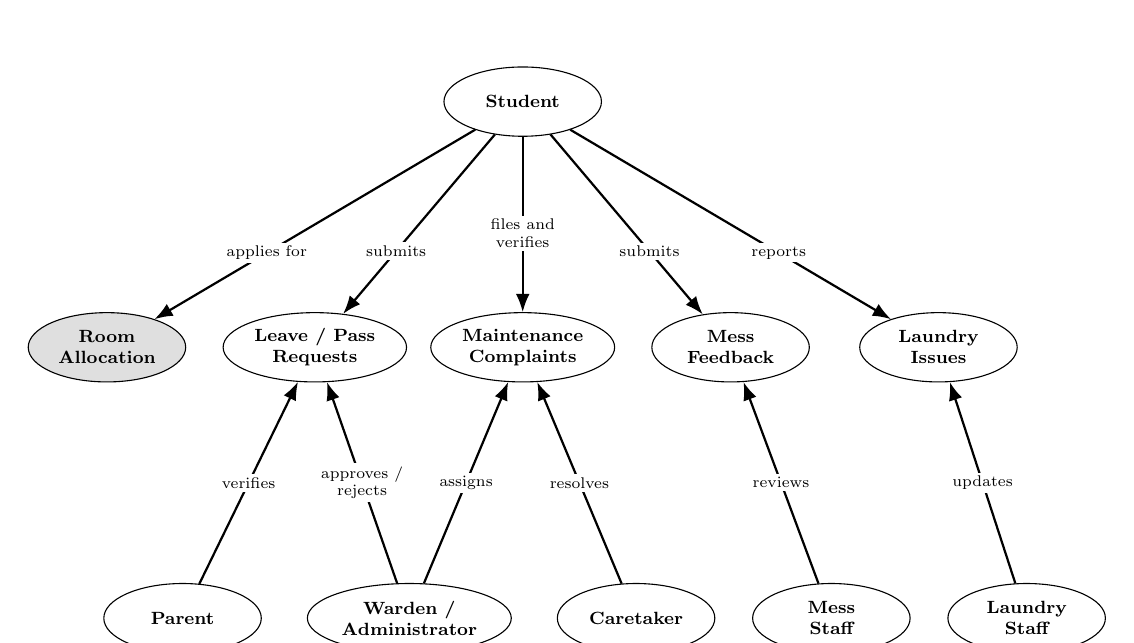
\begin{tikzpicture}[scale=0.8,transform shape,ent/.append style={minimum width=25mm}]
\node[ent] (stu) at (0,0) {Student};
\node[ent,fill=gray!25] (room) at (-6.6,-3.9) {Room\\Allocation};
\node[ent] (leave) at (-3.3,-3.9) {Leave / Pass\\Requests};
\node[ent] (comp) at (0,-3.9) {Maintenance\\Complaints};
\node[ent] (mess) at (3.3,-3.9) {Mess\\Feedback};
\node[ent] (laun) at (6.6,-3.9) {Laundry\\Issues};
\node[ent] (par) at (-5.4,-8.2) {Parent};
\node[ent] (ward) at (-1.8,-8.2) {Warden /\\Administrator};
\node[ent] (care) at (1.8,-8.2) {Caretaker};
\node[ent] (mst) at (4.9,-8.2) {Mess\\Staff};
\node[ent] (lst) at (8.0,-8.2) {Laundry\\Staff};
\draw[flow] (stu) -- node[lbl,pos=0.65]{applies for} (room);
\draw[flow] (stu) -- node[lbl,pos=0.65]{submits} (leave);
\draw[flow] (stu) -- node[lbl,pos=0.55]{files and\\verifies} (comp);
\draw[flow] (stu) -- node[lbl,pos=0.65]{submits} (mess);
\draw[flow] (stu) -- node[lbl,pos=0.65]{reports} (laun);
\draw[flow] (par) -- node[lbl]{verifies} (leave);
\draw[flow] (ward) -- node[lbl]{approves /\\rejects} (leave);
\draw[flow] (ward) -- node[lbl]{assigns} (comp);
\draw[flow] (care) -- node[lbl]{resolves} (comp);
\draw[flow] (mst) -- node[lbl]{reviews} (mess);
\draw[flow] (lst) -- node[lbl]{updates} (laun);
\end{tikzpicture}
\caption{Entire work-flow}
\label{fig:workflow}
\end{figure}

Figure~\ref{fig:workflow} (Entire work-flow) is the overview of the project. The entities depend on one another, which gives a simple picture of the functional activities of the system. In the figure, the shaded entity (Room Allocation) is implemented and all unshaded entities are planned.

\textbf{Student cycle:} a student applies for a room, submits leave requests, files maintenance complaints, submits mess feedback, and reports laundry issues. The student also verifies whether a complaint has really been resolved.

\textbf{Staff and parent cycle:} a parent verifies leave requests of the linked student; the warden approves or rejects leave requests and assigns complaints; the caretaker resolves the assigned complaints; mess staff review mess feedback; laundry staff update laundry issues.

\subsection{Definitions, Acronyms and Abbreviations}
\begin{longtable}{>{\bfseries}p{0.2\textwidth}p{0.72\textwidth}}
\toprule
Term & Meaning\\
\midrule
\endhead
SRS & Software Requirements Specification\\
MVP & Minimum Viable Product: the smallest complete release that delivers the core hostel workflows\\
SLA & Service Level Agreement: the time within which a complaint must be resolved\\
CGPA & Cumulative Grade Point Average\\
API & Application Programming Interface\\
JWT & JSON Web Token, used by the prototype for authentication\\
HTTPS & Hypertext Transfer Protocol Secure\\
Cluster & A group of four students occupying two paired rooms that share a washroom\\
FR & Functional Requirement\\
DFD & Data Flow Diagram: shows how data moves between external entities, processes, and data stores\\
\bottomrule
\end{longtable}

% =====================================================================
\section{Overall Description}
\subsection{Product Perspective}
SHARP is a browser-based web application that replaces paper registers and informal communication in hostel administration. Users interact with role-specific pages, application services process requests, and a database stores user and workflow records. The planned design separates the interface, application/API, workflow services, and persistence layers. The prototype uses Node.js/Express and MongoDB (see Section~\ref{sec:impl}); these are implementation choices and not mandatory product requirements.

\subsection{User Classes and Characteristics}\label{sec:users}
SHARP has the following user classes (Figure~\ref{fig:users}):
\begin{itemize}
\item \textbf{Student:} applies for a room, submits leave requests, maintenance complaints, mess feedback, and laundry issue reports, tracks their status, and verifies complaint resolution.
\item \textbf{Parent:} verifies or declines leave requests linked to their student, where required by hostel policy.
\item \textbf{Warden / Administrator:} approves or rejects leave requests, assigns complaints, and oversees escalations. As the authorized administrator, this role also provisions accounts, assigns roles, and maintains approved workflow settings.
\item \textbf{Caretaker:} accepts assigned maintenance work, updates progress, and records completion.
\item \textbf{Mess Staff:} reviews categorized mess feedback (later phase).
\item \textbf{Laundry Staff:} reviews and updates laundry issue reports (later phase).
\end{itemize}
Access to each record shall be limited by role and, where applicable, by record ownership or assignment.

\begin{figure}[H]
\centering
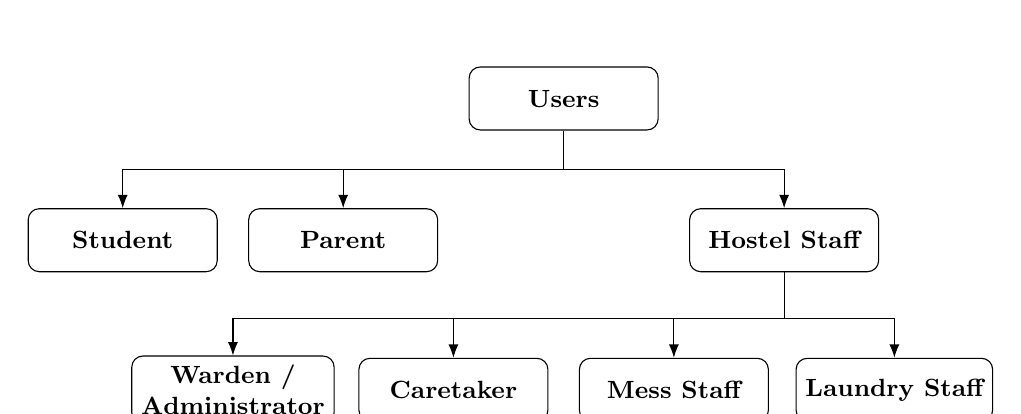
\begin{tikzpicture}
\node[utype] (users) at (0,0) {Users};
\node[utype] (stu) at (-5.6,-1.8) {Student};
\node[utype] (par) at (-2.8,-1.8) {Parent};
\node[utype] (staff) at (2.8,-1.8) {Hostel Staff};
\node[utype] (w) at (-4.2,-3.7) {Warden /\\Administrator};
\node[utype] (c) at (-1.4,-3.7) {Caretaker};
\node[utype] (m) at (1.4,-3.7) {Mess Staff};
\node[utype] (l) at (4.2,-3.7) {Laundry Staff};
\foreach \n in {stu,par,staff}
  \draw[-{Latex}] (users.south) -- (0,-0.9) -| (\n.north);
\foreach \n in {w,c,m,l}
  \draw[-{Latex}] (staff.south) -- (2.8,-2.8) -| (\n.north);
\end{tikzpicture}
\caption{Types of users}
\label{fig:users}
\end{figure}

\subsection{Product Functions}
The main functions of SHARP and their current status are:
\begin{enumerate}
\item \textbf{Portals:} the Student, Parent, and Caretaker portal interfaces have been created; workflows within them may still be incomplete. Warden/Administrator and service-staff interfaces are planned.
\item \textbf{Room allocation (Implemented):} supports cluster/roommate preferences, a cluster leader, three room preferences, and automatic allocation using cluster-average CGPA to resolve conflicts.
\item \textbf{Leave and day-out passes (MVP):} submit requests, record parent verification where required, obtain warden decisions, and issue a digital pass after all required approvals.
\item \textbf{Maintenance complaints (MVP):} submit and assign complaints, track work and SLA deadlines, and close a complaint only after student verification.
\item \textbf{Mess feedback (Planned):} submit categorized feedback and show its content to mess staff without exposing the reporter's identity in ordinary staff views.
\item \textbf{Laundry issue tracking (Planned):} report missing, damaged, incorrect, stained, or delayed items and track their handling status.
\item \textbf{Notifications and reports (Planned, optional):} provide workflow notifications and operational summaries when approved and configured.
\end{enumerate}

Every user has an account with a role. Students additionally belong to a cluster for room allocation.

\textbf{Data flow.} Figure~\ref{fig:dfd0} is the context-level (Level~0) data flow diagram. It shows SHARP as a single process and the data exchanged with each external user class. Figure~\ref{fig:dfd1} is the Level~1 data flow diagram, which splits SHARP into six processes (1.0 to 6.0) and six data stores (D1 to D6). In both figures, rectangles are external entities, rounded rectangles are processes, open-ended rectangles are data stores, and arrows are data flows. A double-headed arrow carries two flows; in its label, $\rightarrow$ marks the flow that moves to the right and $\leftarrow$ the flow that moves to the left. In Figure~\ref{fig:dfd1}, an external entity (for example the Student or the Warden / Administrator) is drawn once for each process it interacts with, only to avoid crossing lines. Of the processes, only 2.0 (room allocation) is implemented, 1.0 is partially built, and 3.0 to 6.0 are planned.

\begin{figure}[H]
\centering
\hyphenpenalty=10000 \exhyphenpenalty=10000 
\resizebox{\linewidth}{!}{%
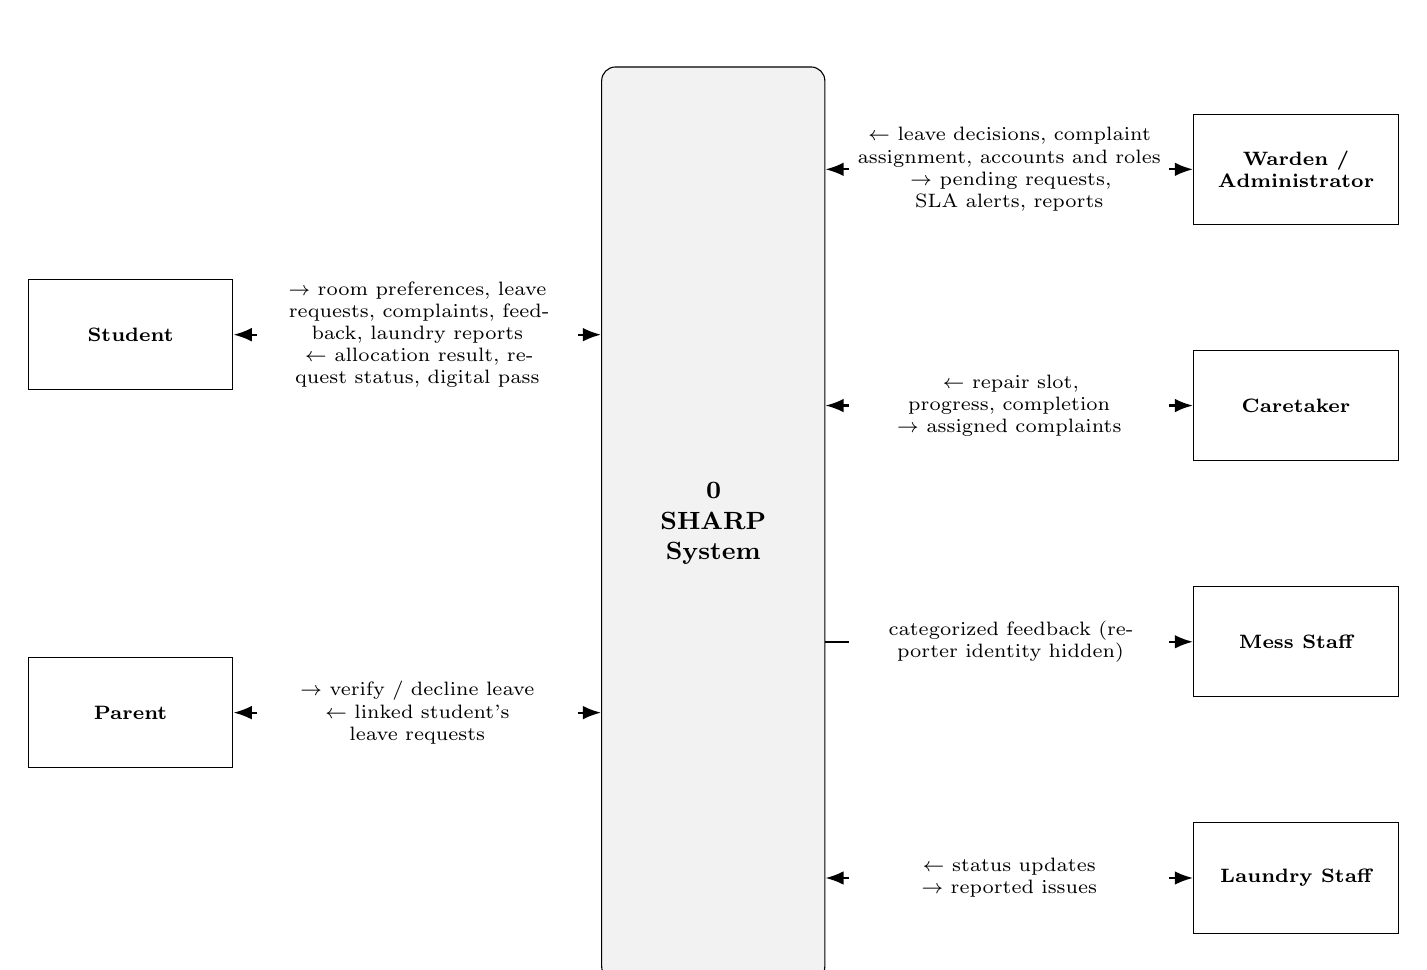
\begin{tikzpicture}[ext/.append style={minimum height=14mm}]
\node[proc,text width=26mm,minimum height=116mm,font=\small\bfseries] (sys) at (0,0) {0\\SHARP\\System};
\node[ext] (stu) at (-7.4,2.4)  {Student};
\node[ext] (par) at (-7.4,-2.4) {Parent};
\node[ext] (war) at (7.4,4.5)   {Warden /\\Administrator};
\node[ext] (car) at (7.4,1.5)   {Caretaker};
\node[ext] (mst) at (7.4,-1.5)  {Mess Staff};
\node[ext] (lst) at (7.4,-4.5)  {Laundry Staff};
\bflow{stu.east}{sys.west |- stu.east}{$\rightarrow$ room preferences, leave requests, complaints, feedback, laundry reports\\$\leftarrow$ allocation result, request status, digital pass}
\bflow{par.east}{sys.west |- par.east}{$\rightarrow$ verify / decline leave\\$\leftarrow$ linked student's leave requests}
\bflow{sys.east |- war.west}{war.west}{$\leftarrow$ leave decisions, complaint assignment, accounts and roles\\$\rightarrow$ pending requests, SLA alerts, reports}
\bflow{sys.east |- car.west}{car.west}{$\leftarrow$ repair slot, progress, completion\\$\rightarrow$ assigned complaints}
\oflow{sys.east |- mst.west}{mst.west}{categorized feedback (reporter identity hidden)}
\bflow{sys.east |- lst.west}{lst.west}{$\leftarrow$ status updates\\$\rightarrow$ reported issues}
\end{tikzpicture}}
\caption{Data Flow Diagram (Level 0)}
\label{fig:dfd0}
\end{figure}

\begin{figure}[H]
\centering
\hyphenpenalty=10000 \exhyphenpenalty=10000 
\resizebox{\linewidth}{!}{%
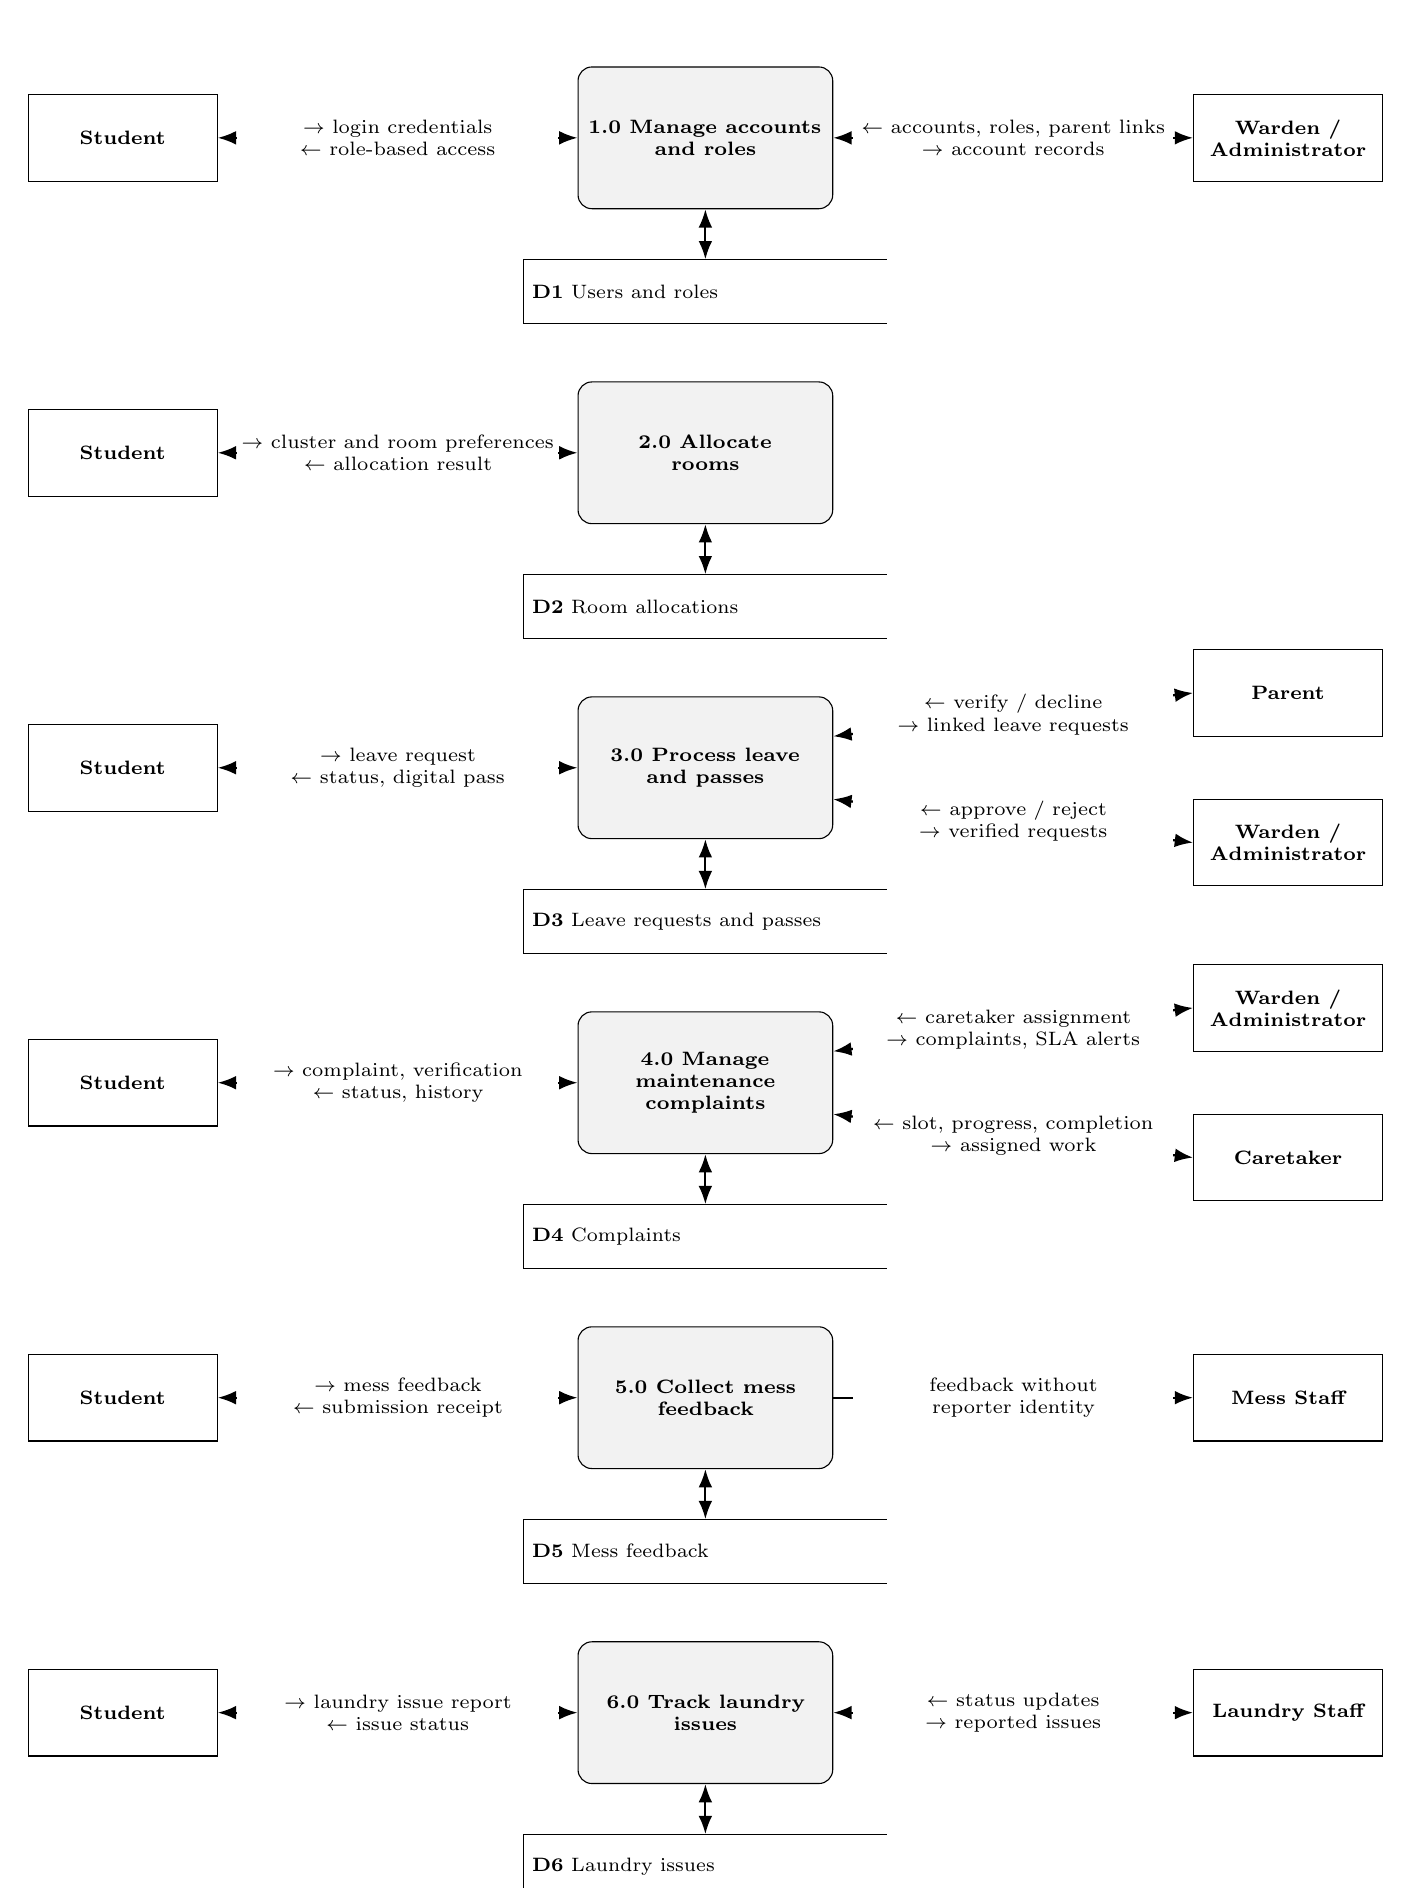
\begin{tikzpicture}[ext/.append style={minimum width=24mm,minimum height=11mm},proc/.append style={text width=30mm}]
% processes (one row each), data store directly below the process
\node[proc] (p1) at (0,0)     {1.0 Manage accounts\\and roles};
\node[proc] (p2) at (0,-4.0)  {2.0 Allocate\\rooms};
\node[proc] (p3) at (0,-8.0)  {3.0 Process leave\\and passes};
\node[proc] (p4) at (0,-12.0) {4.0 Manage maintenance\\complaints};
\node[proc] (p5) at (0,-16.0) {5.0 Collect mess\\feedback};
\node[proc] (p6) at (0,-20.0) {6.0 Track laundry\\issues};
\dstore{d1}{0}{-1.95}  {\textbf{D1}~Users and roles}
\dstore{d2}{0}{-5.95}  {\textbf{D2}~Room allocations}
\dstore{d3}{0}{-9.95}  {\textbf{D3}~Leave requests and passes}
\dstore{d4}{0}{-13.95} {\textbf{D4}~Complaints}
\dstore{d5}{0}{-17.95} {\textbf{D5}~Mess feedback}
\dstore{d6}{0}{-21.95} {\textbf{D6}~Laundry issues}
\foreach \p/\d in {p1/d1,p2/d2,p3/d3,p4/d4,p5/d5,p6/d6}
  {\draw[{Latex}-{Latex},thick] (\p.south) -- (\d.north);}
% Student (repeated for each process)
\foreach \n/\y in {1/0,2/-4,3/-8,4/-12,5/-16,6/-20} {\node[ext] (s\n) at (-7.4,\y) {Student};}
\bflow{s1.east}{p1.west}{$\rightarrow$ login credentials\\$\leftarrow$ role-based access}
\bflow{s2.east}{p2.west}{$\rightarrow$ cluster and room preferences\\$\leftarrow$ allocation result}
\bflow{s3.east}{p3.west}{$\rightarrow$ leave request\\$\leftarrow$ status, digital pass}
\bflow{s4.east}{p4.west}{$\rightarrow$ complaint, verification\\$\leftarrow$ status, history}
\bflow{s5.east}{p5.west}{$\rightarrow$ mess feedback\\$\leftarrow$ submission receipt}
\bflow{s6.east}{p6.west}{$\rightarrow$ laundry issue report\\$\leftarrow$ issue status}
% Staff entities (right)
\node[ext] (w1) at (7.4,0)       {Warden /\\Administrator};
\node[ext] (pa) at (7.4,-7.05)   {Parent};
\node[ext] (w3) at (7.4,-8.95)   {Warden /\\Administrator};
\node[ext] (w4) at (7.4,-11.05)  {Warden /\\Administrator};
\node[ext] (ca) at (7.4,-12.95)  {Caretaker};
\node[ext] (ms) at (7.4,-16)     {Mess Staff};
\node[ext] (ls) at (7.4,-20)     {Laundry Staff};
\bflow{p1.east}{w1.west}{$\leftarrow$ accounts, roles, parent links\\$\rightarrow$ account records}
\bflow{$(p3.east)+(0,0.4)$}{pa.west}{$\leftarrow$ verify / decline\\$\rightarrow$ linked leave requests}
\bflow{$(p3.east)+(0,-0.4)$}{w3.west}{$\leftarrow$ approve / reject\\$\rightarrow$ verified requests}
\bflow{$(p4.east)+(0,0.4)$}{w4.west}{$\leftarrow$ caretaker assignment\\$\rightarrow$ complaints, SLA alerts}
\bflow{$(p4.east)+(0,-0.4)$}{ca.west}{$\leftarrow$ slot, progress, completion\\$\rightarrow$ assigned work}
\oflow{p5.east}{ms.west}{feedback without\\reporter identity}
\bflow{p6.east}{ls.west}{$\leftarrow$ status updates\\$\rightarrow$ reported issues}
\end{tikzpicture}}
\caption{Data Flow Diagram (Level 1)}
\label{fig:dfd1}
\end{figure}

\subsection{Operating Environment}
The system shall be accessed through a modern web browser on a network-connected desktop or mobile device. The server shall run a web application with persistent database storage. The supported browser versions and the hosting environment shall be confirmed before deployment. Offline operation is not required.

\subsection{Design}
The system shall use role-specific pages and forms. Forms shall identify required fields and display validation errors. Users shall be able to view the current status of their own requests and the history permitted by their role.

Student activities have 3 stages (Figure~\ref{fig:student}):
\begin{itemize}
\item Room Allocation Process
\item Service Requests
\item Student Dashboard
\end{itemize}
A student first forms a cluster of four, and the cluster leader submits three room preferences. After the automatic allocation, the student can submit leave requests, complaints, mess feedback and laundry reports, and track or verify them. Every student dashboard contains the allocated room, leave status and digital pass, complaint status, mess feedback and laundry issue status.

\begin{figure}[H]
\centering
\hyphenpenalty=10000 \exhyphenpenalty=10000 
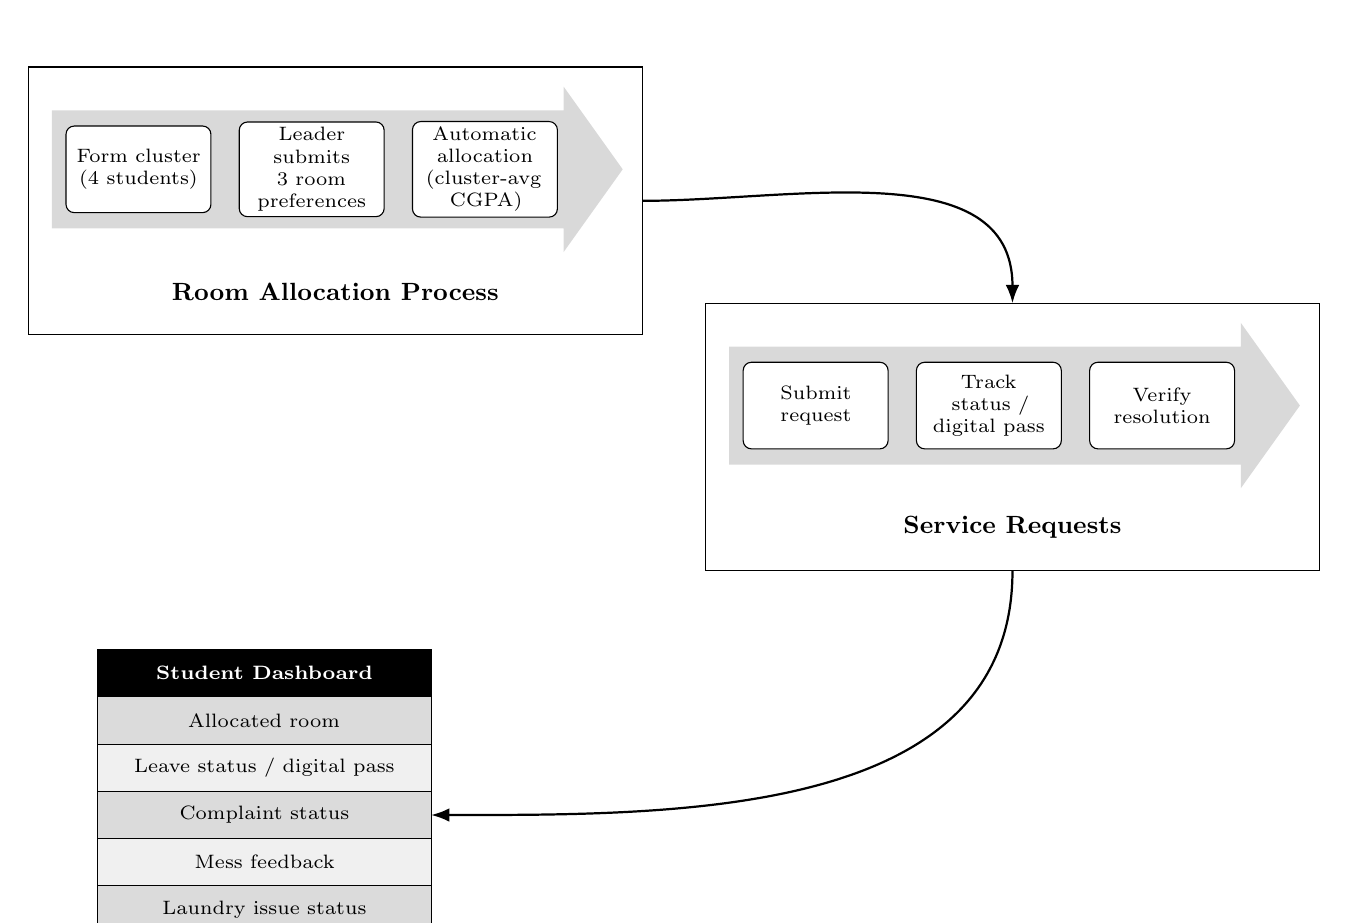
\begin{tikzpicture}
\procbox{b1}{0}{0}{Room Allocation Process}{Form cluster\\(4 students)}{Leader submits\\3 room preferences}{Automatic allocation\\(cluster-avg CGPA)}
\procbox{b2}{8.6}{-3.0}{Service Requests}{Submit request}{Track status /\\digital pass}{Verify\\resolution}
\card{sd}{3.0}{-7.4}{Student Dashboard}{{Allocated room},{Leave status / digital pass},{Complaint status},{Mess feedback},{Laundry issue status}}
\draw[flow] (b1e) to[out=0,in=90] (b2n);
\draw[flow] (b2s) to[out=-90,in=0] (sd3.east);
\end{tikzpicture}
\caption{Student Activities}
\label{fig:student}
\end{figure}

Parent activities (Figure~\ref{fig:parent}) have 2 steps: view the requests of the linked student and verify or decline a leave request.

\begin{figure}[H]
\centering
\hyphenpenalty=10000 \exhyphenpenalty=10000 
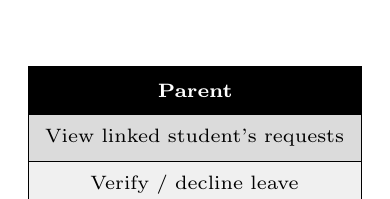
\begin{tikzpicture}
\card{pa}{0}{0}{Parent}{{View linked student's requests},{Verify / decline leave}}
\end{tikzpicture}
\caption{Parent Activities}
\label{fig:parent}
\end{figure}

Hostel staff activities have 2 types (Figure~\ref{fig:hostel}): Warden / Administrator and Caretaker. The Warden / Administrator can approve or reject leave, assign complaints, monitor SLA breaches, provision accounts and roles, and view reports. The caretaker accepts the complaints assigned by the warden, proposes a repair slot, updates progress and marks work complete.

\begin{figure}[H]
\centering
\hyphenpenalty=10000 \exhyphenpenalty=10000 
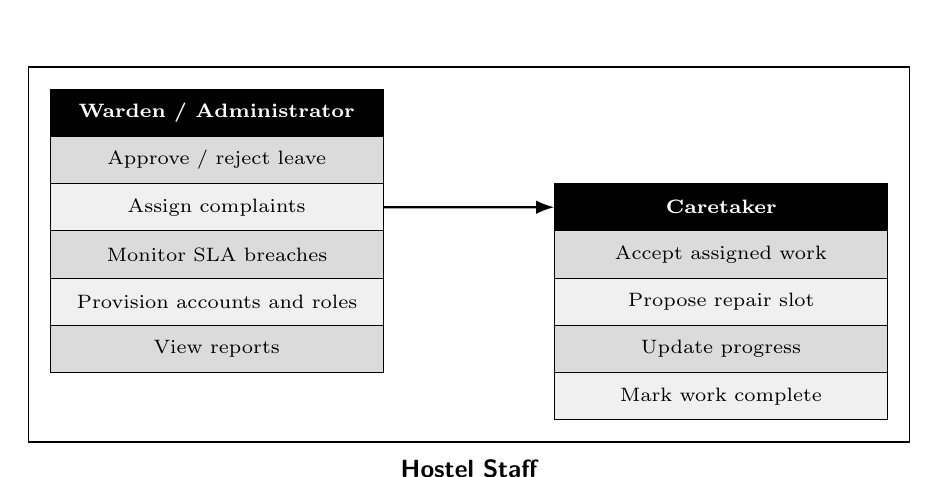
\begin{tikzpicture}
\card{wd}{0}{0}{Warden / Administrator}{{Approve / reject leave},{Assign complaints},{Monitor SLA breaches},{Provision accounts and roles},{View reports}}
\card{ct}{6.4}{-1.2}{Caretaker}{{Accept assigned work},{Propose repair slot},{Update progress},{Mark work complete}}
\draw[flow] (wd2.east) to[out=0,in=180] (cth.west);
\roleframe{(wdh)(wd5)(cth)(ct4)}{Hostel Staff}
\end{tikzpicture}
\caption{Hostel Staff Activities}
\label{fig:hostel}
\end{figure}

Service staff have only one activity each (Figure~\ref{fig:service}): mess staff review categorized feedback, and laundry staff update the status of laundry issues. Both are planned for a later phase.

\begin{figure}[H]
\centering
\hyphenpenalty=10000 \exhyphenpenalty=10000 
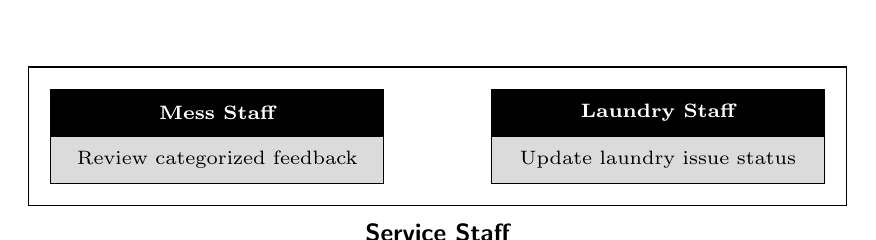
\begin{tikzpicture}
\card{ms}{0}{0}{Mess Staff}{{Review categorized feedback}}
\card{ls}{5.6}{0}{Laundry Staff}{{Update laundry issue status}}
\roleframe{(msh)(ms1)(lsh)(ls1)}{Service Staff}
\end{tikzpicture}
\caption{Service Staff Activities}
\label{fig:service}
\end{figure}

\textbf{Room allocation (implemented).} Users provide roommate/cluster preferences. A cluster contains four students occupying two paired rooms that share a washroom. The cluster leader submits three room preferences, and automatic allocation uses cluster-average CGPA to resolve competing preferences. Further validation and acceptance testing should confirm edge cases and allocation fairness.

\textbf{Leave/pass process (planned).} Student submission, parent verification where required, warden decision, and pass issuance after all required approvals (Figure~\ref{fig:leave}). A rejection at any stage stops the request from proceeding.

\textbf{Complaint process (planned).} Student submission, complaint ID and priority, caretaker assignment, repair-slot agreement (or an alternative slot proposed by the caretaker), repair, and student verification (Figure~\ref{fig:complaint}). Verified complaints are closed; a rejected resolution reopens the same complaint record. An SLA breach notifies the warden.

\begin{figure}[H]
\centering
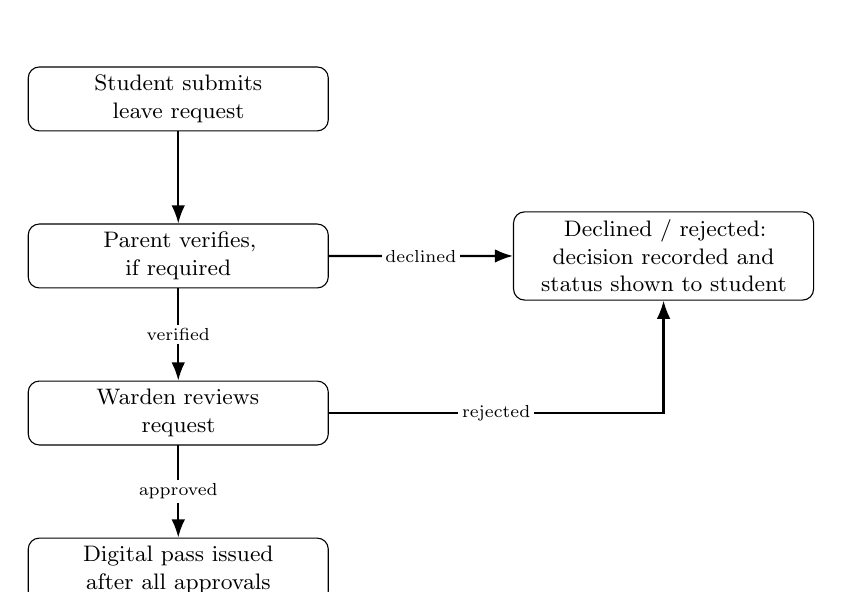
\begin{tikzpicture}[scale=0.9,transform shape,node distance=13mm]
\node[flowbox] (submit) {Student submits\\leave request};
\node[flowbox,below=of submit] (parent) {Parent verifies,\\if required};
\node[flowbox,below=of parent] (warden) {Warden reviews\\request};
\node[flowbox,below=of warden] (pass) {Digital pass issued\\after all approvals};
\node[flowbox,right=26mm of parent] (decline) {Declined / rejected:\\decision recorded and\\status shown to student};
\draw[flow] (submit) -- (parent);
\draw[flow] (parent) -- node[lbl]{verified} (warden);
\draw[flow] (warden) -- node[lbl]{approved} (pass);
\draw[flow] (parent) -- node[lbl]{declined} (decline);
\draw[flow] (warden.east) -| node[lbl,pos=0.25]{rejected} (decline.south);
\end{tikzpicture}
\caption{Leave/pass workflow}
\label{fig:leave}
\end{figure}

\begin{figure}[H]
\centering
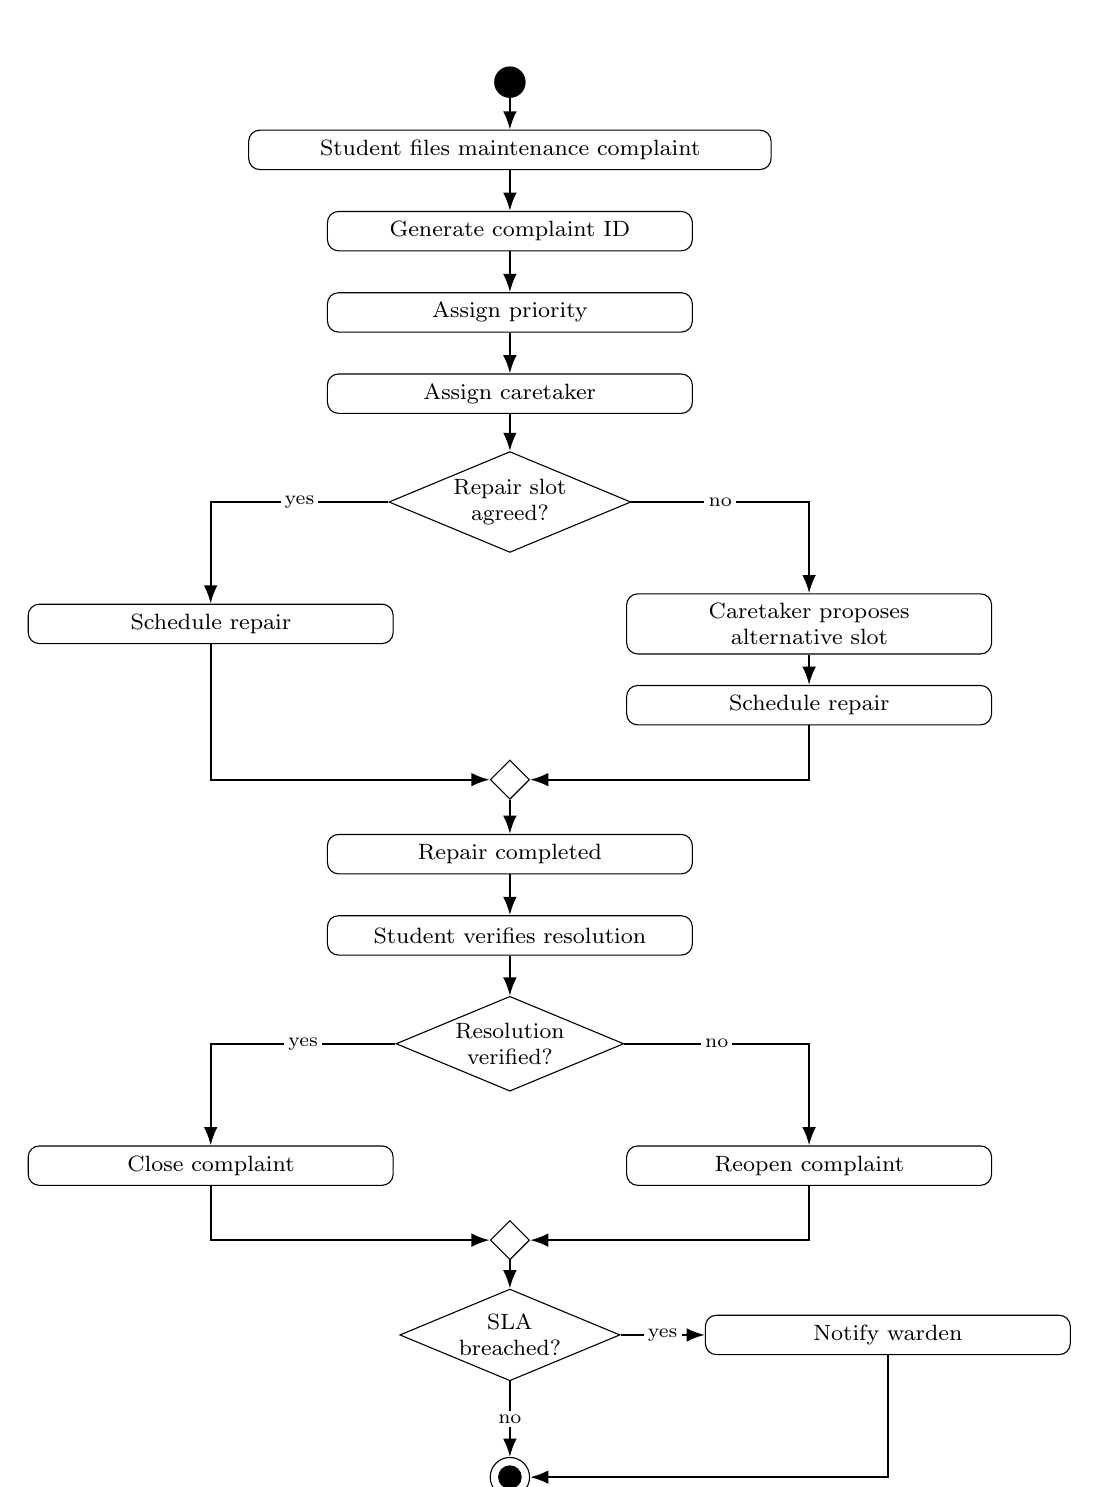
\begin{tikzpicture}[x=1cm,y=0.86cm,flowbox/.append style={minimum height=5mm,font=\footnotesize,text width=44mm},decision/.append style={font=\footnotesize}]
\node[circle,fill=black,minimum size=4mm,inner sep=0pt] (start) at (0,1.0) {};
\node[flowbox,text width=64mm] (c1) at (0,0) {Student files maintenance complaint};
\node[flowbox] (c2) at (0,-1.2) {Generate complaint ID};
\node[flowbox] (c3) at (0,-2.4) {Assign priority};
\node[flowbox] (c4) at (0,-3.6) {Assign caretaker};
\node[decision] (d1) at (0,-5.2) {Repair slot\\agreed?};
\node[flowbox] (s1) at (-3.8,-7.0) {Schedule repair};
\node[flowbox] (a1) at (3.8,-7.0) {Caretaker proposes\\alternative slot};
\node[flowbox] (s2) at (3.8,-8.2) {Schedule repair};
\node[diamond,draw,minimum size=5mm,inner sep=0pt] (m1) at (0,-9.3) {};
\node[flowbox] (c5) at (0,-10.4) {Repair completed};
\node[flowbox] (c6) at (0,-11.6) {Student verifies resolution};
\node[decision] (d2) at (0,-13.2) {Resolution\\verified?};
\node[flowbox] (cl) at (-3.8,-15.0) {Close complaint};
\node[flowbox] (ro) at (3.8,-15.0) {Reopen complaint};
\node[diamond,draw,minimum size=5mm,inner sep=0pt] (m2) at (0,-16.1) {};
\node[decision] (d3) at (0,-17.5) {SLA\\breached?};
\node[flowbox] (nw) at (4.8,-17.5) {Notify warden};
\node[circle,draw,minimum size=5mm,inner sep=0pt] (end) at (0,-19.6) {};
\node[circle,fill=black,minimum size=3mm,inner sep=0pt] at (end) {};
\draw[flow] (start) -- (c1);
\draw[flow] (c1) -- (c2);
\draw[flow] (c2) -- (c3);
\draw[flow] (c3) -- (c4);
\draw[flow] (c4) -- (d1);
\draw[flow] (d1.west) -| node[lbl,pos=0.25]{yes} (s1.north);
\draw[flow] (d1.east) -| node[lbl,pos=0.25]{no} (a1.north);
\draw[flow] (a1) -- (s2);
\draw[flow] (s1.south) |- (m1.west);
\draw[flow] (s2.south) |- (m1.east);
\draw[flow] (m1) -- (c5);
\draw[flow] (c5) -- (c6);
\draw[flow] (c6) -- (d2);
\draw[flow] (d2.west) -| node[lbl,pos=0.25]{yes} (cl.north);
\draw[flow] (d2.east) -| node[lbl,pos=0.25]{no} (ro.north);
\draw[flow] (cl.south) |- (m2.west);
\draw[flow] (ro.south) |- (m2.east);
\draw[flow] (m2) -- (d3);
\draw[flow] (d3.east) -- node[lbl]{yes} (nw.west);
\draw[flow] (d3.south) -- node[lbl]{no} (end);
\draw[flow] (nw.south) |- (end.east);
\end{tikzpicture}
\caption{Maintenance complaint activity diagram}
\label{fig:complaint}
\end{figure}

\FloatBarrier
% =====================================================================
\section{System Features}
SHARP is a hostel workflow platform. Its main purpose is to move the common hostel processes from paper and informal messages into one role-controlled system.

\subsection{Description and Priority}
The table distinguishes the current implementation status from the delivery priority. The portal interfaces exist, but only the room-allocation process is currently implemented. MVP and Planned identify the intended delivery phases, not completed functionality.

\begin{longtable}{>{\raggedright\arraybackslash}p{0.21\textwidth}>{\raggedright\arraybackslash}p{0.41\textwidth}>{\raggedright\arraybackslash}p{0.13\textwidth}>{\raggedright\arraybackslash}p{0.15\textwidth}}
\toprule
\textbf{Feature} & \textbf{Description} & \textbf{Priority} & \textbf{Status}\\
\midrule
\endhead
Portal interfaces & Student, Parent, and Caretaker portals have been created; not all workflows are implemented. & MVP foundation & Partially built\\
Room allocation & Cluster/roommate preferences and CGPA-based automatic allocation. & MVP & Implemented\\
Authentication and roles & Secure sign-in and role/ownership-based access to protected operations. & MVP & Partially built (completeness to be verified)\\
Leave/pass management & Submit leave requests, record required verification and approval, and issue approved passes. & MVP & Not implemented\\
Maintenance complaints & Submit, assign, update, escalate, and verify complaints before closure. & MVP & Not implemented\\
Mess feedback & Collect categorized feedback while hiding reporter identity from ordinary mess-staff views. & Planned & Not implemented\\
Laundry issues & Record and track missing, damaged, incorrect, stained, or delayed items. & Planned & Not implemented\\
Notifications and reports & Optional workflow notifications and administrative summaries. & Planned & Not implemented\\
\bottomrule
\end{longtable}

\subsection{Functional Requirements}
Each functional requirement has an identifier of the form \textbf{FR-\textit{MODULE}-\textit{NN}}, where \textit{MODULE} is a short code for the feature area and \textit{NN} is a two-digit sequence number within that area. The module codes are: AUTH (authentication and access), LEAVE (leave and day-out passes), CMP (maintenance complaints), ROOM (room allocation), MESS (mess feedback), LDRY (laundry issues), NTF (notifications), and RPT (reports). Identifiers are never reused, so they can be referenced from test cases and review comments.

\textbf{Authentication and role access (MVP; portal interfaces created)}
\begin{description}[style=sameline,leftmargin=3.0cm,labelwidth=2.8cm,labelsep=0.2cm,font=\bfseries\small,itemsep=3pt]
\item[FR-AUTH-01] The system shall authenticate users before granting access to protected records or actions.
\item[FR-AUTH-02] The system shall associate each user with an authorized role.
\item[FR-AUTH-03] The system shall check the role and, where applicable, the record ownership or assignment for each protected operation.
\item[FR-AUTH-04] The system shall deny unauthorized access and shall not store credentials in readable form.
\item[FR-AUTH-05] The system shall record significant workflow decisions and status changes with timestamps and the responsible authorized user where applicable.
\item[FR-AUTH-06] Only an authorized administrator (the Warden / Administrator role) shall be able to provision accounts, assign roles, and establish parent--student links.
\end{description}

\textbf{Leave and day-out passes (MVP; not implemented)}
\begin{description}[style=sameline,leftmargin=3.0cm,labelwidth=2.8cm,labelsep=0.2cm,font=\bfseries\small,itemsep=3pt]
\item[FR-LEAVE-01] A student shall be able to submit a leave request with the dates, times, destination, and reason required by hostel policy.
\item[FR-LEAVE-02] The system shall validate required fields and prevent inconsistent date/time ranges.
\item[FR-LEAVE-03] Each request shall receive a unique identifier, a submission timestamp, and a pending status.
\item[FR-LEAVE-04] The system shall route a request for parent verification before warden approval where policy requires it.
\item[FR-LEAVE-05] A linked parent shall be able to verify or decline a request, and the system shall preserve the decision and its timestamp.
\item[FR-LEAVE-06] An authorized warden shall be able to approve or reject a request. A request declined at an earlier required stage shall not proceed to approval.
\item[FR-LEAVE-07] The student and authorized reviewers shall be able to view the current status and decision history.
\item[FR-LEAVE-08] The system shall issue a uniquely referenced digital pass only after all required approvals.
\end{description}

\textbf{Maintenance complaints (MVP; not implemented)}
\begin{description}[style=sameline,leftmargin=3.0cm,labelwidth=2.8cm,labelsep=0.2cm,font=\bfseries\small,itemsep=3pt]
\item[FR-CMP-01] A student shall be able to submit a complaint with a category, description, and preferred repair slot.
\item[FR-CMP-02] Each complaint shall receive a unique identifier, a filing timestamp, and a priority based on configured rules.
\item[FR-CMP-03] An authorized warden shall be able to assign a complaint to a caretaker, and the system shall record the assignment and its time.
\item[FR-CMP-04] The assigned caretaker shall be able to acknowledge the complaint, propose or accept a repair slot, and update progress.
\item[FR-CMP-05] The system shall track the configured SLA deadline and make breached open complaints visible to the warden.
\item[FR-CMP-06] A caretaker shall be able to mark work complete, but this shall not by itself close the complaint.
\item[FR-CMP-07] The student who filed the complaint shall be able to verify or reject the claimed resolution. Verification shall close the complaint; rejection shall reopen the same record and preserve its history.
\item[FR-CMP-08] Students and authorized staff shall be able to view the complaint status and the permitted assignment/status history.
\end{description}

\textbf{Room allocation (Implemented)}
\begin{description}[style=sameline,leftmargin=3.0cm,labelwidth=2.8cm,labelsep=0.2cm,font=\bfseries\small,itemsep=3pt]
\item[FR-ROOM-01] The system shall allow a cluster leader to submit roommate/cluster preferences for a group of four students, according to the allocation rules.
\item[FR-ROOM-02] The allocation process shall support three room preferences for the cluster leader.
\item[FR-ROOM-03] When multiple clusters compete for room preferences, the system shall use cluster-average CGPA as the allocation priority rule.
\item[FR-ROOM-04] The system shall record the resulting room allocation and make the result available to authorized users.
\end{description}

\textbf{Mess feedback, laundry, notifications and reports (Planned)}
\begin{description}[style=sameline,leftmargin=3.0cm,labelwidth=2.8cm,labelsep=0.2cm,font=\bfseries\small,itemsep=3pt]
\item[FR-MESS-01] A student shall be able to submit categorized mess feedback.
\item[FR-MESS-02] Authorized mess staff shall be able to review the feedback content, and ordinary mess-staff views shall not expose the reporter's identity.
\item[FR-LDRY-01] A student shall be able to report a laundry issue and view its status.
\item[FR-LDRY-02] Authorized laundry staff shall be able to update the handling status of a reported issue.
\item[FR-NTF-01] Where an approved notification provider is configured, the system should notify relevant users of workflow events.
\item[FR-RPT-01] Authorized administrative users should be able to view operational summaries based on recorded workflow data.
\end{description}

\subsection{Implementation Requirements}\label{sec:impl}
The application is being developed as a web application with a user interface, an application/API layer, workflow logic, and persistent data storage. The prototype uses a React/Vite frontend, a Node.js/Express backend, MongoDB Atlas, and JWT authentication. This is the current prototype stack; implementation status is recorded separately from the target requirements.

% =====================================================================
\section{Other Nonfunctional Requirements}
\subsection{Performance Requirements}
The following targets are sized for a pilot with a small number of users and shall be checked during testing:
\begin{itemize}
\item Ordinary pages and form submissions should respond within about 3 seconds for up to 20 users using the system at the same time.
\item The room-allocation run for a hostel block should complete within one minute.
\end{itemize}
The test method and results shall be recorded.

\subsection{Security Requirements}
\begin{itemize}
\item Protected actions shall require authentication and server-side authorization.
\item Passwords, if locally managed, shall be stored using a modern salted password-hashing algorithm; plaintext passwords shall not be stored or logged.
\item Production deployment should use HTTPS.
\item Sensitive records shall be visible only to authorized roles and to users with the appropriate record relationship.
\item The mess-feedback reporter's identity shall be hidden from mess staff in ordinary views and service responses.
\end{itemize}

\subsection{Software Quality Attributes}
\begin{itemize}
\item \textbf{Reliability:} successful workflow changes shall persist and be visible on subsequent authorized reads.
\item \textbf{Usability:} forms shall label required fields, explain validation errors, and show the current workflow status.
\item \textbf{Maintainability:} workflow modules should have separable responsibilities and automated tests for critical transitions.
\item \textbf{Compatibility:} the interface should support current stable versions of Chrome, Firefox, and Edge during pilot testing, with responsive layouts at widths of 360 CSS pixels and above.
\item \textbf{Auditability:} important decisions, assignments, status changes, reopenings, and SLA breaches shall retain timestamps and prior history.
\end{itemize}

\subsection{Business Rules}
\begin{itemize}
\item Each request, complaint, pass, or report shall have a unique identifier and a creation timestamp.
\item A digital leave pass shall be issued only after the approvals required by hostel policy.
\item Completion of complaint work and closure of the complaint are separate events; closure requires student verification.
\item A rejected resolution shall reopen the same complaint record rather than create a replacement record.
\item Priority rules, SLA thresholds, leave fields, and approval exceptions shall be configured according to hostel policy.
\item The implemented room-allocation process uses cluster-average CGPA to resolve competing room preferences; the allocation rules should be documented and tested with representative cases.
\item Access to personal records shall be restricted, and retention/deletion periods shall be agreed with institute policy before production use.
\end{itemize}

% =====================================================================
\section{Other Requirements}
SHARP shall be designed so that planned hostel modules can be added without unnecessarily affecting the existing room-allocation process and portal interfaces. The current prototype has the room-allocation process and the Student, Parent, and Caretaker portals; leave/pass processing, complaint management, laundry tracking, mess feedback, notifications, and reporting remain unimplemented. These modules shall be developed and tested before being described as completed.

The following shall be confirmed with the relevant stakeholders before pilot or production use: account provisioning, parent--student linking, leave policies, complaint priorities, SLA thresholds, data retention, notification configuration, and hosting/security responsibilities.

\end{document}
